\documentclass{article}
\usepackage{amsfonts} % For \mathbb
\usepackage{amsmath} % For align*
\usepackage{enumitem} % For customisable list labels
\usepackage{graphicx} % For images
\usepackage{siunitx} % For units
\graphicspath{{./images/}}

\title{University Physics with Modern Physics - Modern Physics by Young and Freedman Notes}
\author{Chris Doble}
\date{June 2023}

\begin{document}

\maketitle

\tableofcontents

\setcounter{section}{16}
\section{Temperature and Heat}

\subsection{Temperature and Thermal Equilibrium}

\begin{itemize}
  \item The \textbf{zeroth law of thermodynamics} states: If $C$ is initially in thermal equilibrium with both $A$ and $B$, then $A$ and $B$ are also in thermal equilibrium with each other.

  \item Two systems are in thermal equilibrium iff they have the same temperature.
\end{itemize}

\subsection{Thermometers and Temperature Scales}

\begin{itemize}
  \item Water freezes at $\ang{0} \unit{C}$ or $\ang{32} \unit{F}$ and boils at $\ang{100} \unit{C}$ or $\ang{212} \unit{F}$.

  \item A temperature measurement is denoted $x \unit{\degree C}$ (``$x$ degrees Celsius'') whereas a temperature interval is denoted $x \unit{C \degree}$ (``$x$ Celsius degrees'').
\end{itemize}

\subsection{Gas Thermometers and the Kelvin Scale}

\begin{itemize}
  \item Under the \textbf{Kelvin} temperature scale temperature differences are equal to those of the degrees Celsius scale, but the zero is equal to $\ang{-273.15} \unit{C}$. This is known as \textbf{absolute zero} where molecules have their lowest possible kinetic and potential energies.

  \item The ratio of two temperatures in the Kelvin scale equals the ratio of the corresponding pressures in a constant-volume gas thermometer \[\frac{T_2}{T_1} = \frac{p_2}{p_1}.\]
\end{itemize}

\subsection{Thermal Expansion}

\begin{itemize}
  \item Materials expand when their temperatures increase.

  \item Expansion in a single dimension is described by the equation \[\Delta L = \alpha L_0 \Delta T\] where $\Delta L$ is the change in length, $\alpha$ is the \textbf{coefficient of linear expansion}, $L_0$ is the original length, and $\Delta T$ is the change in temperature.

  \item Expansion in three dimensions (volume expansion) is described by the equation \[\Delta V = \beta V_0 \Delta T\] where $\Delta V$ is the change in volume, $\beta$ is the \textbf{coefficient of volume expansion} (equal to $3 \alpha$), $V_0$ is the original volume, and $\Delta T$ is the change in temperature.

  \item If the ends of a material are fixed in place, changes in temperature can induce \textbf{thermal stresses} that can damage the material. The magnitude of these stresses is given by \[\frac{F}{A} = -Y \alpha \Delta T.\]
\end{itemize}

\subsection{Quantity of Heat}

\begin{itemize}
  \item Energy transferred as a result of a temperature difference is called \textbf{heat}.

  \item The \textbf{specific heat} of a material is the amount of energy required to raise the temperature of one unit of mass of the material by one unit of temperature, e.g. $\qty{1}{kg}$ by $\qty{1}{K}$. It has units like $\unit{J/(kg.K)}$.

  \item The specific heat of water is \[\qty{4190}{J/(kg.K)} \text{ or } \qty{1}{cal / (g.C\degree)}.\]

  \item The energy required to change the temperature of a material is given by \[Q = m c \Delta T\] where $m$ is the mass of the material, $c$ is its specific heat, and $\Delta T$ is the change in temperature.

  \item The \textbf{molar mass} of a substance is the mass of one mole.

  \item The total mass of a material $m$ is equal to the mass per mole $M$ times the number of moles $n$ \[m = n M.\]

  \item The energy required to change the temperature of a certain number of moles of a substance is \[Q = n C \Delta T\] where $C = M c$ is the \textbf{molar heat capacity}.
\end{itemize}

\subsection{Calorimetry and Phase Changes}

\begin{itemize}
  \item A \textbf{phase} is a specific state of matter, e.g. solid, liquid, or gas.

  \item A \textbf{phase change} or \textbf{phase transition} is a transition from one phase to another.

  \item For a given pressure, phase change takes places at a definite temperature.

  \item While a substance is undergoing a phase change, any added or removed energy will affect the progress of the phase change but won't change the temperature.
\end{itemize}

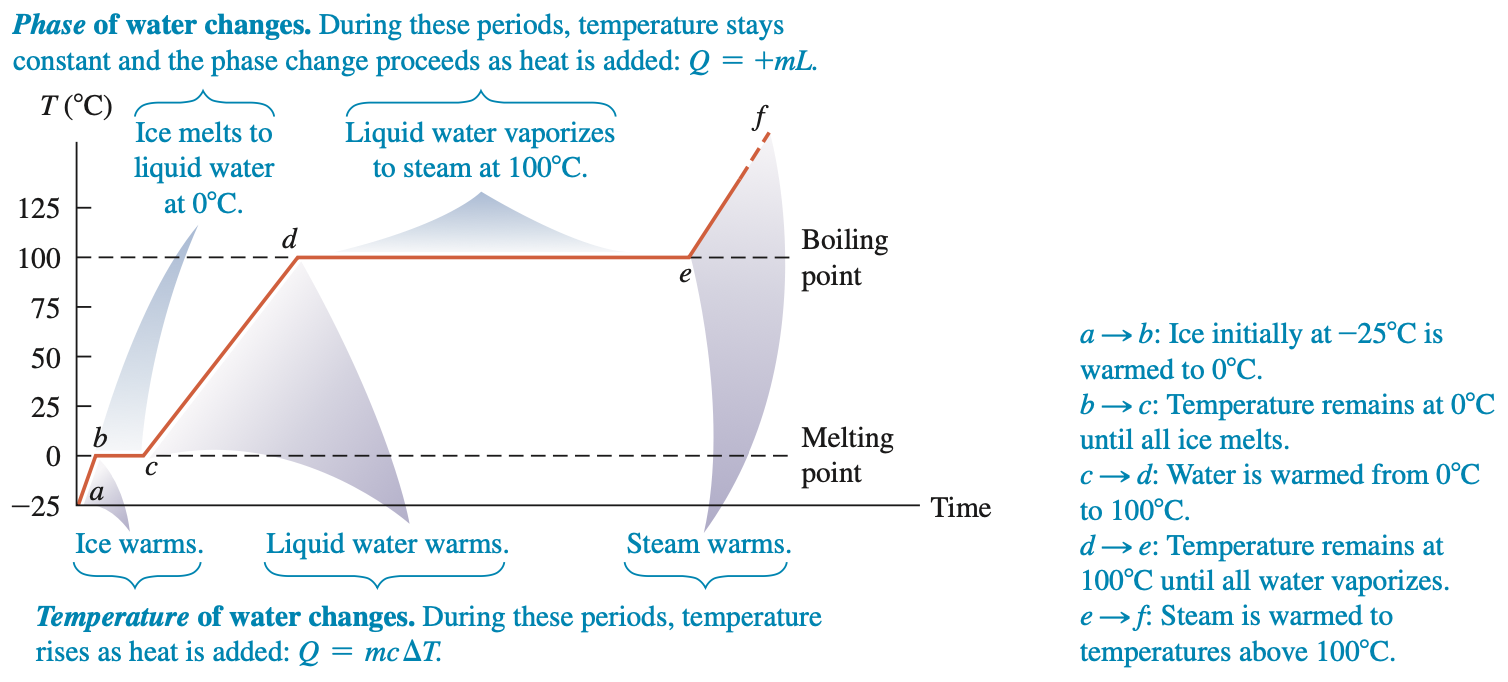
\includegraphics[scale=0.43]{phase-vs-temperature}

\begin{itemize}
  \item The heat transfer required for a material to undergo a phase change is given by \[Q = \pm m L\] where the $\pm$ indicates that heat may need to be added or removed depending on the direction of the phase change (e.g. energy must be added to melt ice), $m$ is the mass of the material, and $L$ is the latent heat associated with the phase change.

  \item When a material is freezing or melting, $L = L_f$ the \textbf{latent heat of fusion}.

  \item When a material is condensing or vaporising, $L = L_v$ the \textbf{latent heat of vaporisation}.

  \item When a material sublimates (changes directly from a solid to a gas, skipping liquid) or deposits/desublimates (changes directly from a gas to a solid, skipping liquid), $L = L_s$ the \textbf{latent heat of sublimation}.

  \item When a material burns, $L = L_c$ the \textbf{latent heat of combustion}.

  \item For any given material at any given pressure, the freezing temperature is the same as the melting temperature. This is called \textbf{phase equilibrium}. Similarly the condensing temperature is the same as the vaporisation temperature.
\end{itemize}

\subsection{Mechanisms of Heat Transfer}

\begin{itemize}
  \item \textbf{Conduction} is a mechanism of heat transfer where the molecules in an area of high temperature have greater kinetic energy, they bump neighboring molecules which increases their kinetic energy, and so on spreading the heat through the material.

  \item The direction of heat flow is always from higher to lower temperature.

  \item When a quantity of heat $dQ$ is transferred through a material in time $dt$ we say the rate of heat flow or the \textbf{heat current} is \[H = \frac{dQ}{dt}.\]

  \item If a rod has cross sectional area $A$, length $L$, one end is held at temperature $T_H$, and the other is held at $T_C$ where $T_H > T_C$, the heat current is \[H = \frac{d Q}{d T} = k A \frac{T_H - T_C}{L}\] where $k$ is the \textbf{thermal conductivity} of the material and $(T_H - T_C) / L$ is the temperature difference per unit length or the magnitude of the \textbf{temperature gradient}.

  \item \textbf{Convection} is the transfer of heat by mass motion of fluid from one region of space to another, e.g. ducted cooling/heating. If the fluid is circulated by a blower or a pump the process is called \textbf{forced convection}; if the flow is caused by differences in density due to thermal expansion, such as hot air rising, the process is called \textbf{free convection}.

  \item \textbf{Radiation} is the transfer of heat by electromagnetic waves such as visible light, infrared, and ultraviolet radiation.

  \item The wavelength of the radiation depends on temperature. At $\qty{20}{\degree C}$ the radiation is infrared. At $\qty{800}{\degree C}$ the radiation is red. At $\qty{3000}{\degree C}$ the radiation is white.

  \item The \textbf{Stefan-Boltzmann law} gives the rate of energy radiation from a surface \[H = A e \sigma T^4\] where $A$ is its surface area, $e$ is a dimensionless constant between 0 and 1 called the \textbf{emissivity} of the surface (1 would be a perfect radiator), $\sigma$ is the \textbf{Stefan-Boltzmann constant} \[\sigma = \qty{5.67037442e-8}{W/(m^2.K^4)},\] and $T$ is the temperature in Kelvin.

  \item An object's surroundings also emit radiation which is absorbed by the object. The net heat current from the object is this \[H = A e \sigma (T^4 - T_s^4)\] where $T_s$ is the temperatue of the surroundings. At thermal equilibrium there is no heat flow.

  \item An object that is a good absorber must also be a good emitter. An ideal radiator with $e = 1$ is also an ideal absorber, absorbing all the raditation that hits it. Such a surface is called an \textbf{ideal black body} or a \textbf{blackbody}.
\end{itemize}

\end{document}